\section{An\'alise dos resultados}
\label{sec:resultados}

% Passa-se ao tratamento dos dados por intermédio dos testes estatísticos, os quais dependem das hipóteses a serem testadas. Nesse tópico, é exigido que sejam aplicados testes de hipóteses paramétricos e/ou não paramétricos. Testes de duas amostras são exigidos quando comparando abordagens

Nessa seção, nós mostramos como tratamos os resíduos dos dados da amostra por intermédio dos testes estatísticos. 

Para interpretar os dados, nós primeiramente conduzimos uma análise descritiva para observar tendência nos dados baseada em algumas características como dispersão e mediana. Nós elaboramos o gráfico Boxplot ilustrado na Figura~\ref{fig:boxplot} para comparar a execução das estratégicas TE e TG. Esse gráfico mostra que o tempo de execução dos testes tende a ser menor para TE. A média para completar as atividades usando TG foi de 975 segundos, enquanto que a média para TG foi de 824 segundos. A TE teve uma diminuição média de 15\% no tempo de execução. No mais, nenhuma discrepância apareceu no gráfico.

\begin{figure}[t]
    \centering
    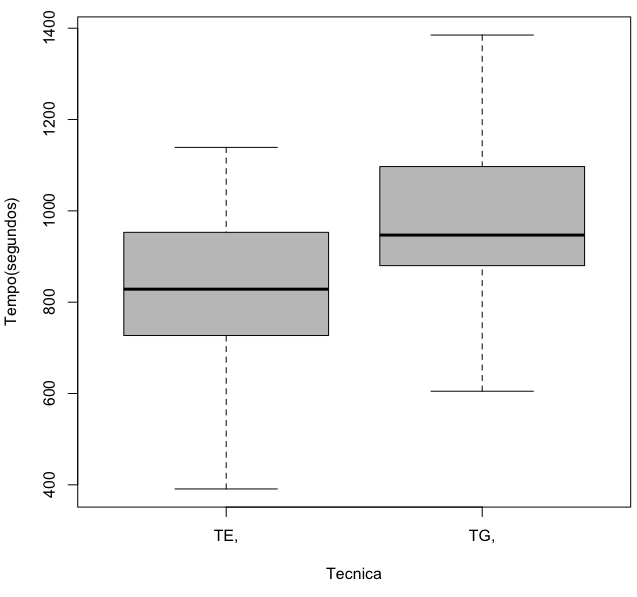
\includegraphics[width=0.4\textwidth]{images/boxplot.png}
    \caption{}
    \label{fig:boxplot}
\end{figure}

% mostrar o dotplot também aqui
Além do Boxplot, nós também elaboramos o gráfico Dotplot ilustrado na Figura~\ref{fig:dotplot} para termos uma visão diferente da análise. Com esse gráfico, podemos ver para cada um dos 18 estudantes, representados de A a R, que o uso da técnica TE (Específico) para executar os testes levou menos tempo do que que TG (Genérico). A única exceção foi o estudante P. Outro ponto importante, é que a feature (F1 ou F2) usada não influencia nos resultados.

\begin{figure}[t]
    \centering
    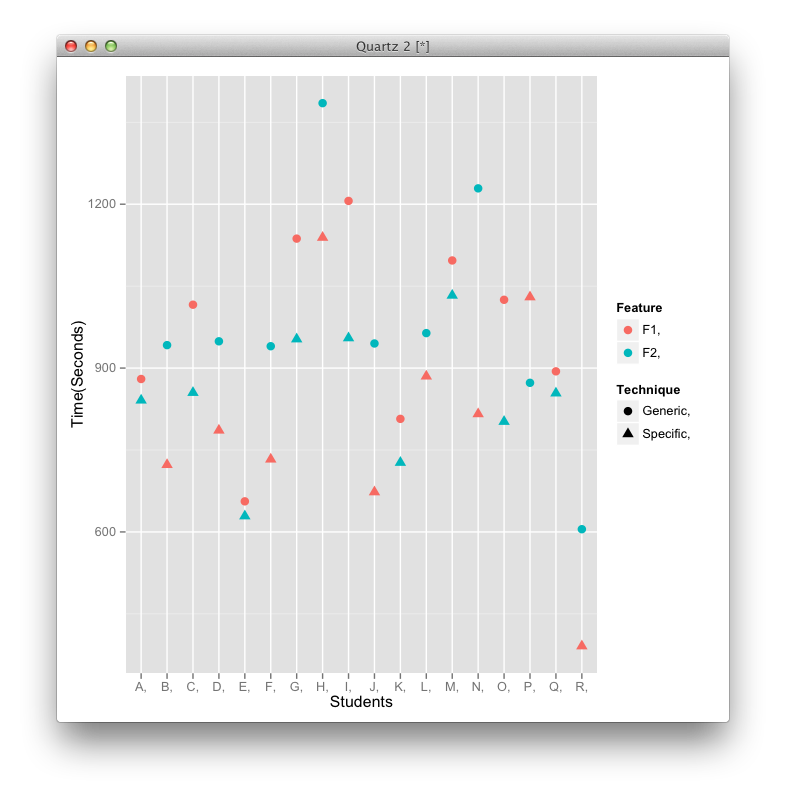
\includegraphics[width=0.4\textwidth]{images/dotplot.png}
    \caption{}
    \label{fig:dotplot}
\end{figure}

Além dos valores da mediana, nós queríamos comparar as observações de acordo com cada resultado das estratégias (TE e TG). Nós pudemos observar para ambas as estratégias que não importa a feature usada para executar os casos de testes, 94\% dos estudantes terminaram em menos tempo usando TE. Dos 18 alunos analisados, só um levou mais tempo para executar os testes com TE.

Continuando com a análise estatística, nós queremos verificar se a tendência observada nas nossas amostras foi de fato significante. Para verificar isso, nós rodamos teste de hipótese paramétrico baseado na média. Nesse contexto, nós usamos o ANOVA como dito na Seção~\ref{sec:metodologia}. Nós executamos o teste ANOVA e alcançamos um \emph{p-value} para o fator da estratégia de aproximadamente 0,0001, o que nos dá evidência significante de que a estratégia TE pode reduzir o tempo de execução das suites de testes.

Todo código escrito em R, dados e fontes do texto podem ser acessados livremente no nosso repositório: \\https://github.com/rcaa/ProjetoEstatistica2013